\chapter{General discussion}
\label{ch:generaldiscussion}

\section{Contributions of this thesis}

This thesis aimed to investigate the microbial ecology and biogeography of the \ac{SO}.
To achieve this, two factors that structure the biogeographic distribution of microorganisms in the \ac{SO} were selected for study: the \ac{PF}, a major biogeographic barrier, and advection, a potentially major biogeographic force.

\subsection{The Polar Front}

This project found good evidence that the \ac{PF} is a major biogeographic barrier in the \ac{SO}, by demonstrating that the bacterial and archaeal communities in the waters to the south (the \ac{AZ}) are significantly different from the waters to the north (the \ac{SAZ} and subtropical waters north of the \ac{STF}, primarily representing \ac{SAMW}) (\secreft{ch:polarfront}).

This is not the first study on the effect of the \ac{PF} on the distribution of \ac{SO} microbiota.
Variation in the position of the \ac{ACC}, which determines the location of the \ac{PF}, has been shown to influence zooplankton composition \citep[e.g.][]{Chiba:2001un,Hunt:2001vp}, including dinoflagellates \cite{Esper:2002ui}\footnote{Interestingly, one study described the biogeographic effect of \ac{ACC}-associated fronts on zooplankton as being only weakly related to environmental parameters \cite{Ward:2003db}, suggesting the effect of advection (\secreft{ch:advection}) on zooplankton as a potential avenue for future research}.
The \ac{ACC} and/or \ac{PF} have similarly been shown to influence the distribution of Roseobacter phylotypes \cite{Selje:2004ka,Giebel:2009hr}, Flavobacteria \cite{Abell:2005ji}, and SAR11 phylotypes \cite{Giebel:2009hr}.
However, this thesis provides a significant contribution, presenting the first community-level (metagenomic) survey of \ac{SO} bacterial and archaeal plankton performed over a latitudinal transect occupying all major \ac{SO} surface water masses to give an integrated snapshot of the microbial ecology and biogeography of the \ac{SO}.

As well as the confirming previous findings on the level of individual taxonomic groups, this study found that the effect of the \ac{PF} extends to the whole community, and even to the distribution of genomically encoded functional potential.
The higher abundance south of the \ac{PF} of Bacteroidetes and Rhodobacterales, associated with the degradation of phytoplanktonic byproducts \citep[e.g.][]{Buchan:2005hd,Williams:2012gsa}, reflect the higher concentrations of (primarily eukaryotic) phytoplankton in this region. 
This was also reflected in the functional analysis, with an overrepresentation of high-specificity transporters, suggestive of copiotrophic taxa in a ``feast'' phase \cite{Lauro:2009gx}.
In general, waters south of the \ac{PF} reflected the upwelling of nutrient-rich \ac{NADW} and higher supply of light during the austral summer, which make the region significantly more active and productive than \ac{SAZ} and even subtropical waters to the north.

These northern waters were characterised by a higher relative abundance of slow-growing, nutrient-scavenging oligotrophs such as SAR11 and SAR116.
Functionally, this was reflected in the higher abundance of genes encoding branched-chain amino acid transporters, which both SAR11 and SAR116 possess.
The other significant feature of region north of the \ac{PF} was the higher abundance of the cyanobacterial genera \genus{Prochlorococcus} and \genus{Synechococcus}, and concurrently the photosynthesis functions they encode.
This was most likely due to the sensitivity of these genera to temperature.

\subsubsection{Biogeographic role of the Polar Front}

Having shown that the \ac{PF} is a major biogeographic barrier, and in light of the advection study also presented in this thesis (\secreft{ch:advection}), it is worth considering the mechanism(s) by which the \ac{PF} shapes microbial biogeography.
It is likely that three main forces are at work.

The first is the role of the \ac{PF} as a ``biogeographic barrier'' in the classical sense in which the term is applied to macroorganisms.
In other words, it physically prevents or slows the migration of cells between the regions it divides, leading if not to allopatric speciation, at least to some degree of genetic divergence, which is amplified by the differences in environmental properties.
\citet{Selje:2004ka}, who first reported that \ac{RCA} phylotypes differed across the \ac{PF}, offered this mechanism as a likely explanation, an idea corroborated by further reports on RCA \cite{Giebel:2009hr} and Flavobacteria \cite{Abell:2005ji}.
The advection effect (\secreft{ch:advection}) supports such a mechanism, by showing that oceanic regions poorly connected by advection (i.e.\ poorly mixed) have less similar microbial communities.

The second mechanism, complementary to the first, is the difference in physicochemical properties resulting from the same oceanographic forces that create the \ac{PF}: in particular, the advective distribution of nutrients.
The ratio of biological N/P export in \ac{SO} surface waters increases northwards from the region of upwelling \ac{CDW} in the \ac{AZ} (N/P\textsubscript{exp} \textless{} 16) to the \ac{SAZ} (N/P\textsubscript{exp} \textgreater{} 16) \cite{Weber:2010fi}.
This directly contradicts the standard assumption that \ce{PO4^3-} is exported to the deep ocean in a fixed proportion of \textapprox{}16:1 available \ce{NO3^-} to \ce{PO4^3-} (the Redfield ratio).
\citet{Weber:2010fi} convincingly showed that this is largely a result of the biogeographic distribution of low cellular N/P diatoms relative to other high cellular N/P plankton.
The distribution of diatoms in the \ac{SO} is in turn controlled by the concentration of silicic acid \cite{MFranck:2000kt}, which supplied in abundance south of the \ac{PF} by upwelling \ac{CDW} but is limiting further north \citep[widely held, but well summarised by][]{Coale:2004to}, explaining the observed difference in N/P\textsubscript{exp}.
Further, \citet{Weber:2010fi} showed that advective mixing of organic N and P exported to the deep ocean by sinking organic matter and remineralised in the aphotic zone was sufficient to counterbalance the differential export of N and P by diatoms and other plankton, leading to an equilibrium approximately equivalent to the Redfield ratio of 16:1 N:P.
Advective transport of nutrients and the distribution of plankton are thus intimately connected in the \ac{SO}, with the \ac{PF} acting as a key barrier between the nutrient-rich \ac{AZ} upwelling and the comparatively oligotrophic \ac{SAZ}.
As well as the distribution of these major nutrients (N, P and Si), the waters to the north and south of the \ac{PF} differ in temperature and salinity due to their different circulatory origins \cite{Foldvik:1988gp}.

The third mechanism by which the \ac{PF} may act as a biogeographic boundary is more mundane.
Being a polar ocean, the \ac{SO} is subject to strong latitudinal gradients in air temperature and sunlight unrelated to its oceanographic structure.
The Antarctic Circle, the latitude at which continuous 24-hour periods of sunlight (and of darkness) become possible, is considerably south of the \ac{PF} (\textapprox{}66.5\textdegree{} S, although this varies due to slow changes in the Earth's axial tilt).
However, the existence of large environmental gradients means that longitudinal features (fronts, currents, divergences and convergences in both the ocean and atmosphere) are almost certain to be associated with biological discontinuities simply by virtue of lying on a particular latitude, without necessarily having any causal relationship.
In the case of the \ac{PF} and its role in the distribution of marine bacteria and archaea, the possibility that this was the only significance of the \ac{PF} was explicitly tested for and discounted in this study: other arbitrary latitudinal lines do not structure the biological observations as well as the \ac{PF} (see \secreft{ch:polarfront}).
Nevertheless, it is likely that latitudinal gradients not directly related to the \ac{PF} (particularly sunlight) do make some contribution to the biogeographic pattern.

\subsubsection{The Polar Front and climate change}

Global climate change is already having a large effect on the \ac{SO}.
The \ac{ACC} is largely driven by the strong westerly winds that are characteristic of sub-polar Ferrel cells in atmospheric circulation.
The \ac{SAM} (also known as the Antarctic Oscillation) is a complex, low-frequency oscillation in the latitude and speed of this westerly wind belt between ``positive'' (further south, stronger flow) and ''negative'' (further north, weaker flow) phases.
As a result of climate change, the long-term trend of the \ac{SAM} may be towards the positive phase \cite{Thompson:2002ic}.
Along with an increase in the temperature of \ac{ACC} waters (also due to climate change \cite{Aoki:2003fo,Boning:2008il}), this may be responsible for the observed southward migration of the mean position of the \ac{ACC} by \textapprox{}50 km since the 1950s \cite{Gille:2002fr}.
Even with optimistic assumptions about future anthropogenic greenhouse gas emissions, it has been predicted to move a further \textapprox{}1.4\textdegree{} south (\textapprox{}150 km) by the year 2100 \cite{Fyfe:2005vp}.

The effects of climate change on marine ecology are often thought of in terms of changes in physicochemical properties such as temperature, salinity, pH, and atmospheric \ce{CO_{2}}.
However, changes to the location of biogeographic barriers such as the \ac{PF} may also be significant.
Southward migration of the \ac{PF} will displace a large surface area of \ac{AZ} waters enriched by upwelling nutrients, increasing the relative area of the comparatively oligotrophic \ac{SAZ}.
This may result in a net decrease in primary production, although concurrent changes in temperature and other physicochemical properties make this difficult to predict.
As the \ac{SO} is a major site for sequestration of anthropogenic \ce{CO_2} through the biological pump \cite{Thomalla:2011hi}, this raises the possibility of creating a negative feedback loop \cite{Cox:2000ko} which would further accelerate global climate change.

\subsubsection{Future work}

One of the limitations of the \ac{PF} study was the latitudinal coverage provided by the sample sites.
While this was sufficient to investigate the biogeographic role of the \ac{PF}, it was not fine-scaled enough to conclusively resolve the effects of other fronts.
Moreover, the study only examined surface waters.
A large-scale gridded (latitude, longitude and depth) survey would be of enormous value in linking \ac{SO} microbial communities to their oceanographic context.
Regular samples from the same stations over an annual cycle would also be useful in establishing seasonal changes.

The expense and logistical difficulty of sampling in the \ac{SO}, especially in higher latitudes and during winter months, are a major challenge for future metagenomic surveys.
Current progress on autonomous \textit{in situ} microbial sampling and analysis instruments \cite{CSIRO:2012uw} has the potential to reduce these limitations and provide a robust platform for future work.
These platforms aim to replicate the enormous success of the global Argo network of autonomous oceanographic floats, by combining instrumentation for simple abiotic measurements with the automatic filter collection and storage of seawater biomass for later retrieval and metagenomic analysis.
\textit{In situ} community analysis, for example with onboard microfluidics and a DNA microarray system such as PhyloChip (Berkeley Lab, Berkeley, USA) are also under consideration \cite{CSIRO:2012uw}.
A network of even a small number of these probes could quickly exceed shipboard sampling efforts at a lower cost, and provide better coverage of logistically difficult regions and times of year in the \ac{SO}.

An advantage of the shotgun metagenomic approach as employed in the \ac{PF} study is the ability to identify the functional potential of sampled microorganisms, as revealed by their encoded genes.
However, genomic potential is only a window into the actual ecological function of microbes: it does not take into account levels of transcription and translation, nor differences in these levels between cells in a clonal population.
Recent work on biofilms has clearly demonstrated that even genomically identical bacteria can ``differentiate'' in a way analogous to cells in a multicellular organism when those bacteria form environmental consortia \cite{Sauer:2002ux}.
The size fractionation approach provides an excellent opportunity to compare the expression profiles of planktonic and particle-attached \citep[i.e.\ potentially biofilm-forming; see][]{Grossart:2003uv} phases in the marine context.
Future work integrating metagenomic and metaproteomic analyses with size fractionation would be of great value in expanding our understanding of the ecosystem processes performed by \ac{SO} microorganisms.

\subsection{The advection effect}

The second major focus of this thesis was the role of advection in shaping the biogeography of microorganisms in the \ac{SO}, and by extension the ocean in general.
This question is highly topical, given the recent discovery that geographic distance often controls microbial biogeography in contradiction with the Baas Becking hypothesis (key studies: \citet{Cho:2000tn,Whitaker:2003dz}; reviews: \citet{Martiny:2006jy,Hanson:2012cb}), and the frequent invocation of circulation to explain observed distributions of marine microbes \citep[e.g.][]{Lauro:2007bf,Giebel:2009hr,Ghiglione:2012ei,Sul:2013in}.

Previous work addressing this question has focused on water mass endemicity and qualitative descriptions of circulation.
\citet{Galand:2009hy} and \citet{Agogue:2011fm} presented evidence of the specificity of microbial communities to water masses in the Arctic and North Atlantic oceans, even across small geographic distances, suggesting boundaries between water masses act as biogeographic barriers, although these observations do not exclude simple environmental selection.
\citet{Hamilton:2008tp}, also describing the Arctic and North Atlantic oceans, found picoeukaryotic communities clustered by circulatory origin as determined by qualitative analysis of hydrographic properties.
The authors noted that quantitative modelling of circulation would be necessary to directly test the role of circulation.
Recently, \citet{Hamdan:2013ko} demonstrated a similar clustering of prokaryotes Arctic marine sediments with their circulatory origins.
Both studies controlled for environmental factors to various degrees.

This thesis (and the associated publication) present the first quantitative test of the effect of advection on microbial biogeography.
By employing a high-resolution computational model of \ac{SO} circulation to determine advective distances between samples, the standard ecological tools of distance matrices and partitioning of variance with the partial Mantel test could be used to isolate the effect of advection from environmental selection and spatial separation.
This thesis thus also contributes a replicable method for future studies to evaluate the advection effect in other marine environments and directly compare it to other biogeographic forces.

\begin{figure}
  \centering
  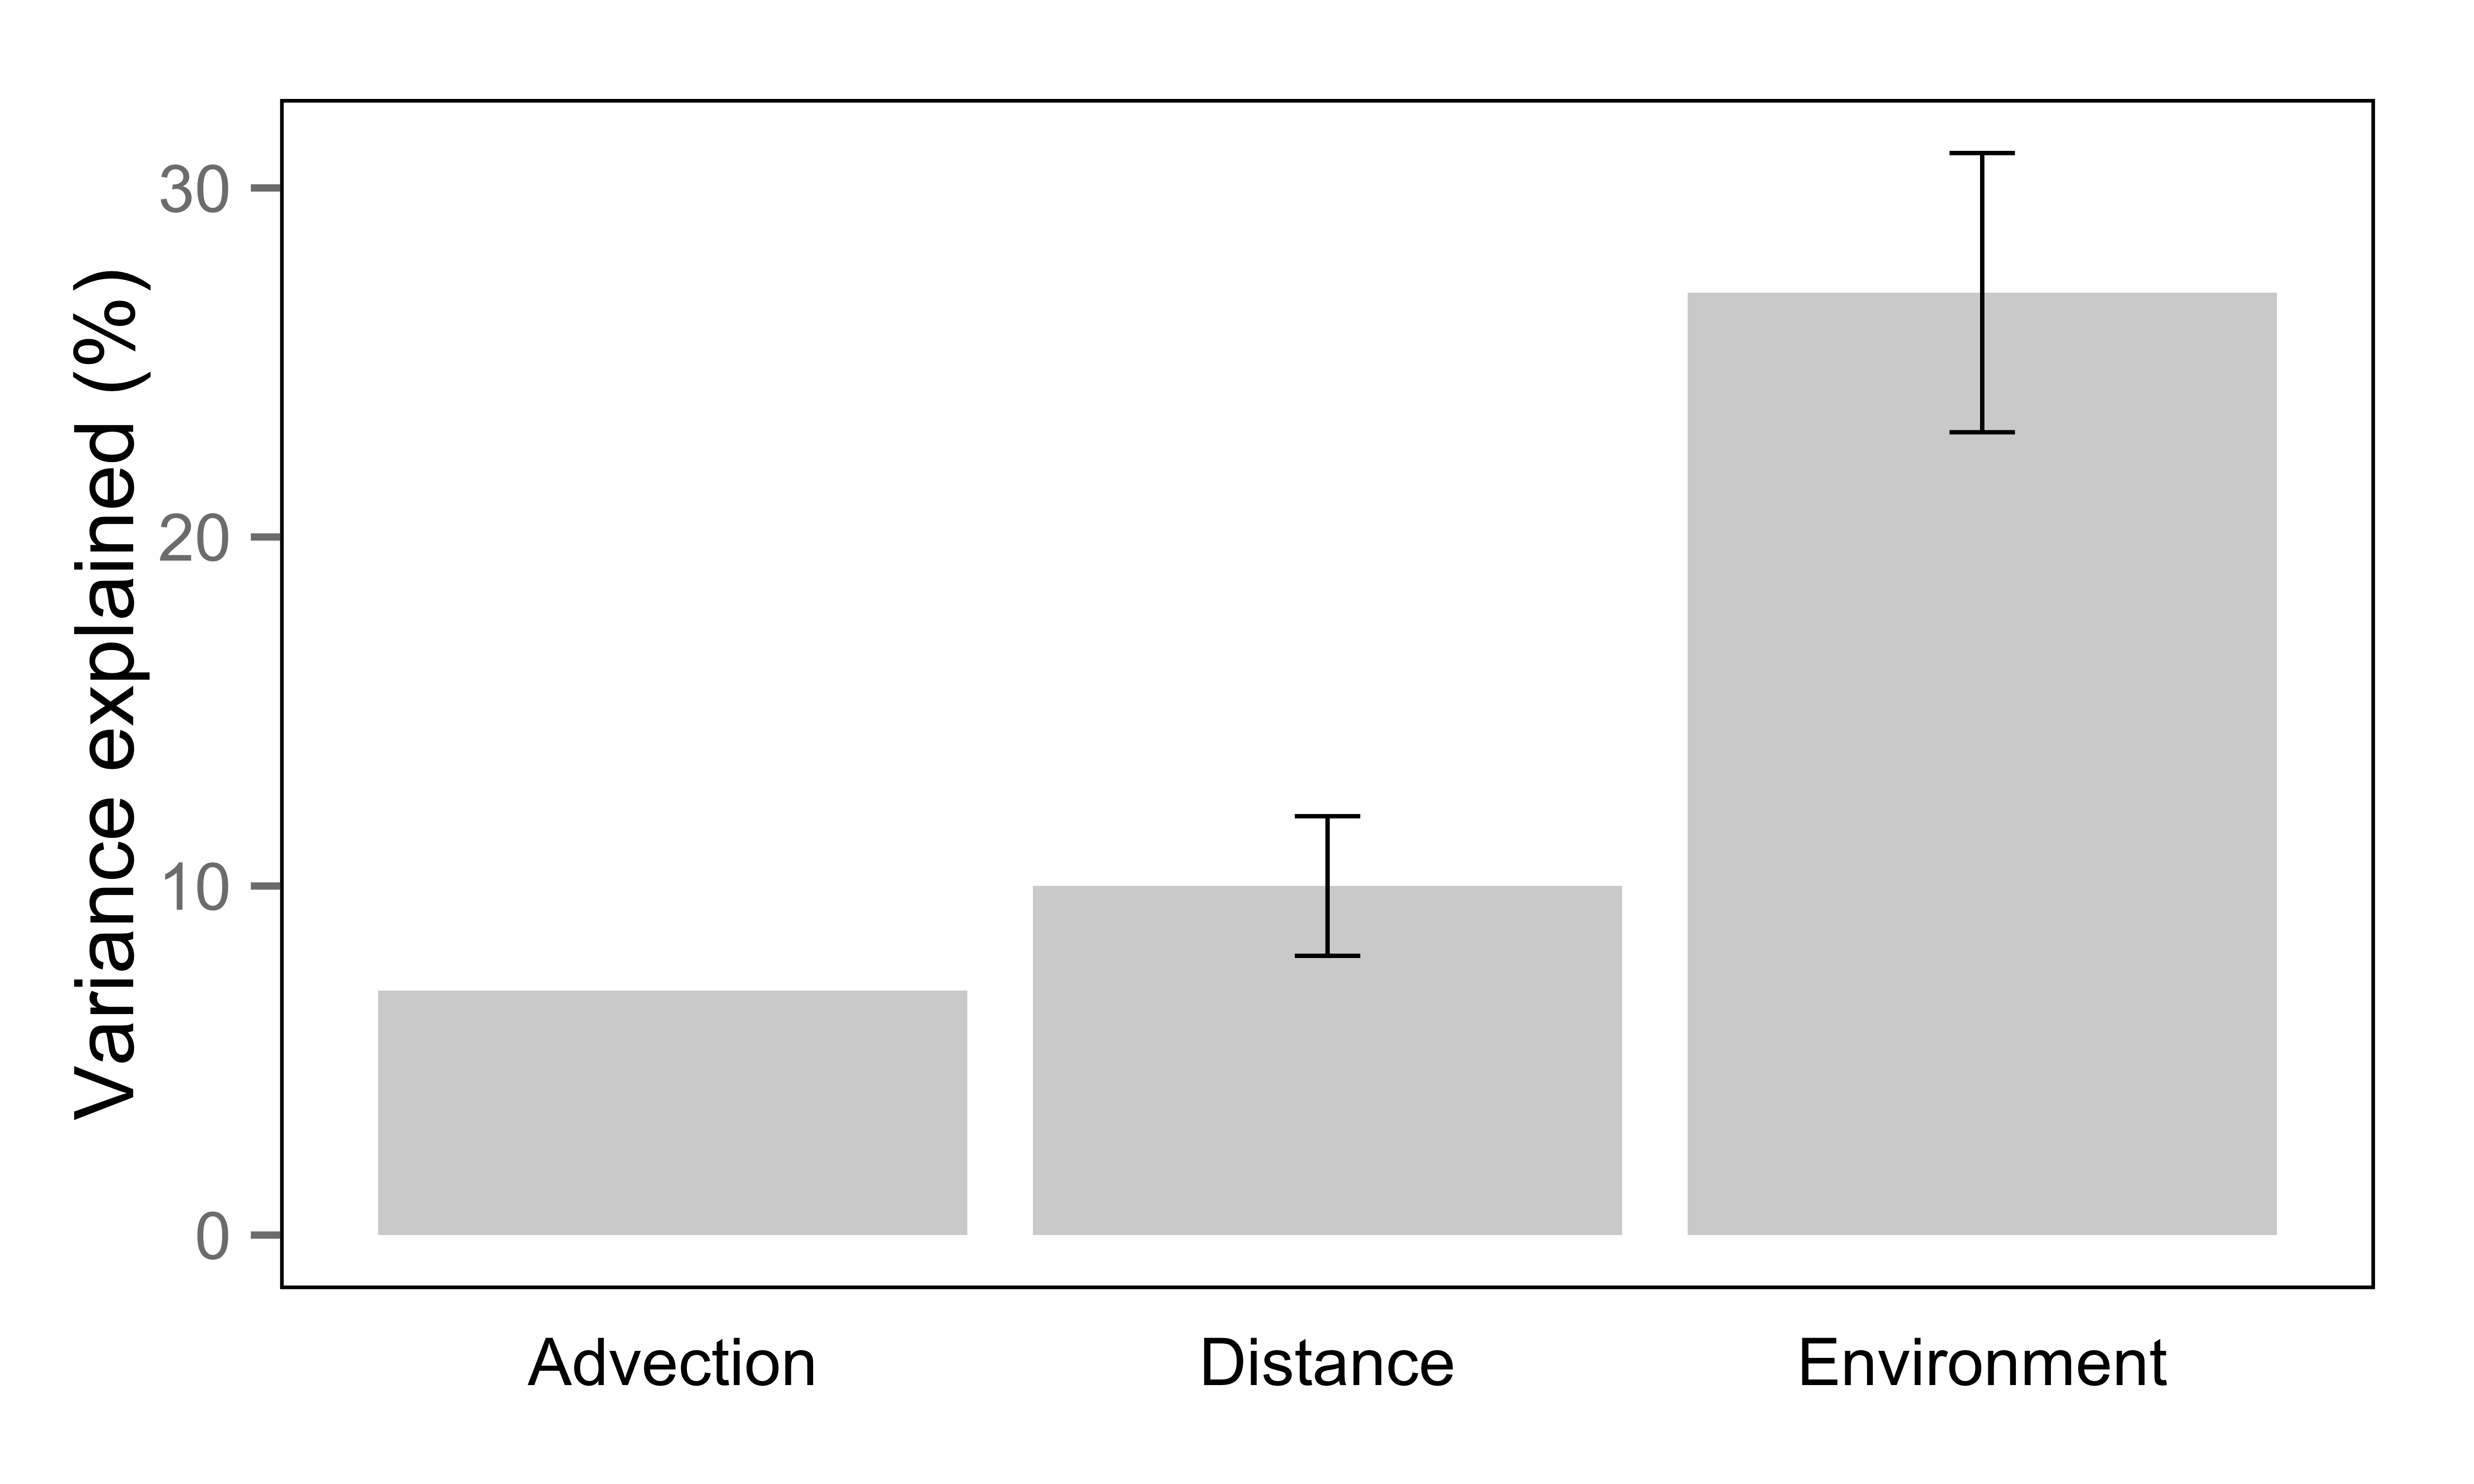
\includegraphics[width=\textwidth]{../generaldiscussion/biogeographybarchart.png}
  \caption[Biogeographic effect sizes]{Variation in microbial community composition explained by environment and distance effects (data from review of 19 studies by \citet{Hanson:2012cb}; error bars represent standard error) and by the advection effect (this study).}
  \label{fig:biogeographybarchart}
\end{figure}


Together, contemporary environmental selection and geographic distance explain \textapprox{} 50\% of variation in microbial community composition \cite{Hanson:2012cb}.
In this study, advection was estimated to explain 7\% of variation \figref{fig:biogeographybarchart}.
This is a conservative estimate, as higher values were found when alternative distance metrics were considered and problematic samples excluded, and samples which shared a common advective origin but had a large mutual advective distance were not considered.

\subsubsection{Future work}

The immediate need for future work on the advection effect is replication, to confirm its existence and measure its magnitude in other oceanic regions.
It is also important that potential alternative explanations for the results, such as the existence of a hidden physicochemical variable (e.g.\ pH, iron concentration) are eliminated by experiments which include measurement of these potential confounds.

Following this, there are several interesting open questions regarding the effect.
In the study described in this thesis, an attempt was made to identify a subset of \acp{OTU} which were more strongly affected by advection than the full set, potentially due to increased resistance to environmental stress and an ability to remain viable over longer distances and times \cite{Bissett:2010wj}.
While such subsets were indeed identified, their biological significance remained ambiguous.
Future work could address this question either by refinement of the statistical methods or with \textit{in vitro} studies of candidate organisms.
While \textit{in situ} cell tracking experiments using the addition of tracer radioisotopes (e.g.\ \ce{^{13}C}) are probably not feasible, it may be possible to use natural radionuclides (e.g.\ \ce{^{234}Th} \cite{Savoye:2005ck} or atmospheric \ce{^{7}Be} \cite{Feng:1999ww}) to the same effect for at least some cell types.

Another question is the effect of advection on organisms other than the 0.1--20 \micron{} bacteria and archaea considered in this study.
The addition of unicellular eukaryotes to the community analysis would be valuable.
Even more interesting would be the effect of advection on marine viruses: bacteriophage have been described as major reservoirs of genetic diversity in the ocean \cite{Suttle:2005bs}, and exchange of genes between phage and host populations may be very common and responsible for the enormous geographic range of identical phage genes \citep[reviewed in][]{Hambly:2005cm}.
However, many virions are labile in the ocean, particularly in surface waters where they are exposed to ultraviolet light, raising the possibility that advection of bacterial cells may be a vehicle for dispersal of viruses or virus genes across long distances.
Understanding the role of advection in spreading microbial diversity therefore require integrating models of physical transport with gene flow.

\subsection{\softwarename{minspec}}

This thesis also presents a novel software tool, \softwarename{minspec}, which contributes to improving the accuracy of \ac{OTU} assignment and calculation of relative abundances in metagenomic studies.

The number of publicly available full genome sequences for microbial species is growing exponentially: over the course of this project, the number of microbial genomes in the RefSeq database increased from 5,500 (May 2010) to 15,000 (March 2013) (\url{http://www.ncbi.nlm.nih.gov/refseq/statistics/}, accessed 12 April 2013).
As more genomes become available, the number of potential high-quality matches to a given metagenomic read will increase as a natural result of genomic identity between related organisms.
\softwarename{minspec} reduces the need to rely on nucleotide identity as the sole objective standard for assigning metagenomic reads to \acp{OTU}, making use of the contextual information provided by the full set of reads to inform the assignment of each individual read.
While assembly of metagenomic reads can to some extent perform the same function \cite{Temperton:2012fj}, \softwarename{minspec} does not require long or overlapping reads, making it well-suited to the short read lengths of current next-generation sequencing methods and to environments such as the open ocean that have a long tail of low-abundance taxa.

In the long term, single-cell genomic sequencing is the most promising approach for accurate and reliable environmental genomics \cite{Blainey:2013dp}.
Until then, \softwarename{minspec} may be of use in improving the quality of metagenomic results.

\section{The species concept in the ``omics'' age}

In some fortunate disciplines, the natural ontologies by which humans ``carve up'' the observed world into conceptual units map well onto the underlying phenomena.
In medicine, for example, the object of study (the human body) is physically divided into easily recognised and discrete units (organs) which have likewise discrete and well-defined functions.
A physician's mental model of the human body has familiar and tangible components, and allows them to understand diseases as systematic divergences from the body's normal form and function.
In physics, on the other hand, such intuitive ontologies frequently fail and even mislead.
The vision of electrons as discrete spheres orbiting a nucleus like planets around a star holds a strong intuitive appeal, but is contradicted by wave-particle duality, and any physicist who failed to resist this tempting but incorrect view would be at an enormous disadvantage.
Physicists, unlike physicians, must either work in new and unfamiliar modes of thinking, or abandon a conceptual grasp of their objects of study altogether and instead investigate them indirectly through mathematical surrogates.

In microbiology, the natural unit of study is the cell, and the natural unit by which cells are categorised is the species.
Although defining microbial species is not quite as straightforward as for sexually reproducing macroorganisms, the usual standards of 16S and genomic similarity are sufficient for laboratory experiments involving clonal or simple mixed populations in culture.
Environmental microbiologists, in need of a similar unit of categorisation but faced with the diversity and depth of environmental populations, frequently use the \ac{OTU} as a practical method of categorising cells with properties similar enough for the purposes of the scientific question at hand.

The rapidly emerging ``omics'' approaches to environmental microbiology have begun to strain the limits of this view.
Enormous population sizes, short generation times and the high rate of horizontal gene transfer between bacterial cells mean that rather than discrete numbers of distinct \acp{OTU}, environmental assemblages may be better described as ``a continuum of genomic possibilities'' \cite{Goldenfeld:2007im}.
Just as a physicist may know that electrons are not infinitesimal billiard balls, but still struggle to conceptualise the wave function of a fundamental particle as anything other than a mathematical abstraction, attempting to describe the ecological and biogeographic patterns of environmental microbes with the familiar vocabulary of species (or \acp{OTU}) and cells can be challenging.
This has been illustrated many times during the course of this thesis.
In the study of the \ac{PF} (\secreft{ch:polarfront}), a large and statistically significant difference between the communities to the north and south of the front was found to be driven by a long and flat distribution of \acp{OTU}, each of which individually contributed only a small amount of variance \tabref{tab:otussimper}.
Likewise, the differences in functional potential between the zones were spread thin over a large number of functional gene categories \tabref{tab:modulessimper,tab:orthologsimper} which nevertheless represented a real and important distinction \textit{in toto}.
In \secreft{ch:advection}, the attempt to identify \acp{OTU} which differentially contributed to the statistically well-supported advection effect yielded results in the form of subsets of \acp{OTU} that were best correlated with the effect.
However, the biological relevance of these subsets was not clear.

It may simply be unfruitful to try to conceptualise such patterns on the level of individual \acp{OTU}.
Instead, continued progress towards a complete 

TODO need some more detail here on what the "new vision" actually looks like, more simulation less "simpler reasoning" 

The recent renewal of activity in microbial biogeography \cite{Ramette:2006jo}, the urgency of climate change and other ecological problems and the improvement in technologies for interrogating environmental assemblages all create a need to develop ways of meaningfully describing, categorising and drawing conclusions from environmental data \cite{Goldenfeld:2007im}.
As in physics, this may require the reluctant abandonment of intuitive and straightforward conceptual models for a less familiar but more accurate ontology.
Mathematics has benefited in the last four decades from the advent of ``computer-assisted proofs'', which are frequently incomprehensible to human workers but are nevertheless valid and allow progress in otherwise moribund lines of enquiry \citep[most famously, the proof of the Kepler conjecture by][]{Hales:2005um}.
The rapidly increasing volume and complexity of environmental genomic data may mean microbiologists will have to accept a similar trade-off: relinquishing the familiar divisions of cells and species in exchange for more accurate models of microbial ecosystems.

\section{Conclusions}
This project has demonstrated the role of the \ac{PF} as a major biogeographic barrier in the \ac{SO}.
It has also provided the first direct evidence that the advection of marine microbes influences their community composition.
As well as these results, this thesis contributes methodological advances with the metagenomic tool \softwarename{minspec} and a replicable method for assessing the advection effect in marine systems.
Increased knowledge about fundamental patterns in microbial ecology and biogeography, as well as the specific ecosystem of the \ac{SO}, will be valuable to shaping our response to ecological challenges such as climate change and expanding our understanding of microbial life on Earth.
